%2multibyte Version: 5.50.0.2953 CodePage: 1252
% green
% blue
% orange
% purple
% red
% resets numbering each section

\ifdefined\extendedversion\else
  \PassOptionsToClass{handout}{beamer}
\fi
\documentclass[xcolor=x11names,compress,aspectratio=169]{beamer}%
\usepackage{amsmath}
\usepackage{amsfonts}
\usepackage{amssymb}
\usepackage{graphicx}
\usepackage{tikz}
\usepackage{pgfplots}
\pgfplotsset{compat=1.18}
\usepackage{dcolumn}%
\setcounter{MaxMatrixCols}{30}
%TCIDATA{OutputFilter=latex2.dll}
%TCIDATA{Version=5.50.0.2953}
%TCIDATA{Codepage=1252}
%TCIDATA{CSTFile=beamer.cst}
%TCIDATA{Created=Monday, May 13, 2013 15:44:12}
%TCIDATA{LastRevised=Tuesday, October 07, 2025 13:11:39}
%TCIDATA{<META NAME="GraphicsSave" CONTENT="32">}
%TCIDATA{<META NAME="SaveForMode" CONTENT="1">}
%TCIDATA{BibliographyScheme=Manual}
%TCIDATA{<META NAME="DocumentShell" CONTENT="Other Documents\SW\Slides - Beamer">}
%TCIDATA{Language=American English}
%BeginMSIPreambleData
\providecommand{\U}[1]{\protect\rule{.1in}{.1in}}
%EndMSIPreambleData
%\usepackage{etex} %vers l'infini et au-dela
\usepackage{minted}
\beamertemplatenavigationsymbolsempty
\usepackage[utf8]{inputenc} 
\usepackage[T1]{fontenc} % pour taper les lettres accentuees
%\usepackage[francais, english]{babel} %le rapport est en franÁais 
\usepackage{amsthm,amssymb,amsbsy,amsmath,amsfonts,amscd,mathrsfs}
\usepackage{geometry} %pour la modification des marges
%\usepackage{fancyhdr} %pour modification des pieds de page
%\usepackage{lastpage} %numero de la derniËre page
\usepackage{lmodern}
\usepackage{lscape} % Pour pouvoir activer le mode landscape
\usepackage{booktabs} %tableaux
\usepackage{float}	%pour forcer le placement des images.
\usepackage{graphicx} %pour afficher des images
\usepackage{longtable} %tables sur plusieurs pages
\usepackage{animate} %transformer des gifs
\usepackage{caption}
\captionsetup{labelformat=simple}
\setbeamertemplate{caption}[numbered]
\setbeamerfont{caption}{size=\scriptsize}
\usepackage[scriptsize]{subfigure}
\usepackage{multirow} 			%fusionner lignes
\usepackage{tikz}
\usepackage{adjustbox}
\usetikzlibrary{arrows,positioning}
\usetikzlibrary{mindmap,trees,shadows,backgrounds}
\usepackage{tabularx}
\usepackage{verbatim}%insertion de code
\usepackage{listings}
\usepackage{dsfont} % Pour les lettres mathematiques
\usepackage{hyperref} %pour que les references soient des liens hypertextes
\usepackage{natbib}
\usepackage{bibentry}
\usepackage{color}
\definecolor{bg}{rgb}{0.95,0.95,0.95}

\def\LECTURENAME{Mod\'elisation, estimation, simulation des risques climatiques}
\def\DIPLOMA{Master in Economics, 2$^{nd}$ year}
\def\UNIV{Ecole Polytechnique}
\def\WEBPAGE{\href{http://vermandel.fr/btm/}{http://vermandel.fr/btm}}
\def\SHORTNAME{Modélisation, estimation, simulation des risques climatiques}



%\usepackage{mathpazo}
\usepackage{multimedia}
\usepackage{dcolumn}
\usepackage{mathtools}
\usepackage{xspace}
\usepackage{array}%

\usepackage{graphicx}

\definecolor{light-gray}{gray}{0.85}
\usepackage{ragged2e} % Pour justifier
\definecolor{bleu}{RGB}{0,129,188}
\definecolor{rouge}{RGB}{238,50,78}
\definecolor{orange}{RGB}{255,100,0}
\definecolor{vert}{RGB}{0,157,87}
\newtheorem{hypothese}{Hypoth\`ese}
\newtheorem{remarque}{Hypoth\`ese}
\newtheorem{theoreme}{Th\'eor\`eme}[section]
\newtheorem{definitionDeux}{D\'efinition}[section]
\newcommand{\iid}{\stackrel{\mathrm{iid}}{\sim}}
\usepackage[official,right]{eurosym} % symbols euro
\usepackage{gensymb} % symbole degre \degre
\usepackage{eurosym} % symbole euro
\usepackage{rotating}
\usepackage{multicol}

% Bibliographie
%\usepackage{bib entry}
%\nobibliography*
%\let\newblock\relax

%\usepackage[notocbib]{apacite}
%\usepackage[style=apa]{biblatex}
%\usepackage[round]{natbib}
%\usepackage[style=authoryear]{biblatex}
%\usepackage[backend=bibtex, style=authoryear-comp]{biblatex}
%\usepackage{biblatex}
%\renewcommand*{\bibfont}{\scriptsize} % Pour avoir la biblio en plus petit
%\usepackage{apacite}
%\bibliographystyle{apacite}

\justifying %on justifie le texte du document
\definecolor{deepblue}{RGB}{0,129,188}
\definecolor{deepblue2}{RGB}{158, 64, 57}
\definecolor{deepblue3}{RGB}{245, 84, 66}


% Pour l'annexe (http://tex.stackexchange.com/questions/2541/beamer-frame-numbering-in-appendix)
\newcommand{\backupbegin}{
   \newcounter{framenumberappendix}
   \setcounter{framenumberappendix}{\value{framenumber}}
}
\newcommand{\backupend}{
   \addtocounter{framenumberappendix}{-\value{framenumber}}
   \addtocounter{framenumber}{\value{framenumberappendix}} 
}

%\usepackage{epstopdf}
%\epstopdfDeclareGraphicsRule{.gif}{png}{.png}{%
%  convert gif:#1 png:\OutputFile
%}
%\AppendGraphicsExtensions{.gif}

% A NE PAS UTILISER !
%\let\olditem=\item% 
%\renewcommand{\item}{\olditem \justifying}%

\justifying

%\graphicspath{{../images}}


\usepackage{dcolumn}


% THEME %
\usetheme{Frankfurt}
\useoutertheme[subsection=false,shadow]{miniframes}

\addtobeamertemplate{background canvas}{\transfade[duration=.3]}{}

% Fonts
%\usefonttheme[onlymath]{serif}
%\usefonttheme{structuresmallcapsserif}
%\usefonttheme[onlymath]{mathserif}
%\usefonttheme{serif}
\setbeamerfont{section in head/foot}{size=\tiny, shape=\normalfont}
\setbeamerfont{subsection in toc}{shape=\normalfont, size = \scriptsize}
\setbeamerfont{section in toc}{size = \small, shape=\normalfont}
% Colours
\setbeamercolor{section in head/foot}{fg=black, bg=gray!5}
\setbeamercolor{frametitle}{bg=white, fg=black}
\setbeamercolor{lower separation line head}{bg=black!5}

\setbeamertemplate{sections/subsections in toc}[square]
\setbeamertemplate{items}[triangle]
\setbeamertemplate{itemize subitem}[triangle]
\setbeamertemplate{itemize subsubitem}[ball]
\setbeamertemplate{enumerate items}[default]
\setbeamertemplate{frametitle}[default][rounded=false,shadow=true]

\setbeamercovered{transparent}



\usepackage{assets/beamerouterthemeEwen}
\usepackage{assets/beamercolorthemeEwen}
\usepackage{assets/beamerhighlight}


\newcommand*\grasO[1]{\textbf{\textcolor{orange}{#1}}} 
\newcommand*\grasR[1]{\textbf{\textcolor{rouge}{#1}}}
\newcommand*\grasV[1]{\textbf{\textcolor{vert}{#1}}} 
\newcommand*\grasB[1]{\textbf{\textcolor{bleu}{#1}}} 


\definecolor{rcp26}{RGB}{39, 55, 122}
\definecolor{rcp45}{RGB}{112, 159, 200}
\definecolor{rcp60}{RGB}{222, 99, 43}
\definecolor{rcp85}{RGB}{205, 16, 32}
\definecolor{dp}{RGB}{181, 73, 60}

\newcommand*\grasRCPa[1]{\textbf{\textcolor{rcp26}{#1}}}
\newcommand*\grasRCPb[1]{\textbf{\textcolor{rcp45}{#1}}} 
\newcommand*\grasRCPc[1]{\textbf{\textcolor{rcp60}{#1}}} 
\newcommand*\grasRCPd[1]{\textbf{\textcolor{rcp85}{#1}}} 
%\newcommand {\red} {\color{red}}
\newcommand {\white} {\color{white}}
%\newcommand {\black} {\color{black}}
\def\Frac#1#2{ #1 \color{red}\above 0.4pt \normalcolor #2}


\usetikzlibrary{decorations}
\usetikzlibrary{decorations.pathmorphing}
\usetikzlibrary{shapes.geometric}
\usetikzlibrary{calc}
\usetikzlibrary{decorations.fractals}
\useoutertheme[subsection=false,shadow]{miniframes}
\useinnertheme{default}
\usefonttheme{serif}
\setbeamerfont{title like}{shape=\scshape}
\setbeamerfont{frametitle}{shape=\scshape}
\setbeamercolor*{lower separation line head}{bg=DeepSkyBlue4}
\setbeamercolor*{normal text}{fg=black,bg=white}
\setbeamercolor*{alerted text}{fg=dp}
\setbeamercolor*{example text}{fg=black}
\setbeamercolor*{structure}{fg=black}
\setbeamercolor*{palette tertiary}{fg=black,bg=black!10}
\setbeamercolor*{palette quaternary}{fg=black,bg=black!10}
\renewcommand{\(}{\begin{columns}}
\renewcommand{\)}{\end{columns}}
\newcommand{\<}[1]{\begin{column}{#1}}
\renewcommand{\>}{\end{column}}
\setbeamertemplate{navigation symbols}{}
\setbeamertemplate{headline}{}
\setbeamertemplate{footline}
{
\leavevmode
\hbox{\begin{beamercolorbox}[wd=1\paperwidth,ht=2.25ex,dp=1ex,center]{title in head/foot}\usebeamerfont{title in head/foot}\hfill\hspace*{12em}\insertshorttitle\hspace*{3em}
\insertframenumber{} / \inserttotalframenumber\hspace*{1ex}
\end{beamercolorbox}}
\vskip0pt
}
\newcommand {\red} {\color{red}}
\newcommand {\black} {\color{black}}
\newcommand{\green}{\color{green}}
\definecolor{deepblue}{RGB}{0,129,188}
\newcommand{\pink}{\color{magenta}}
\newcommand{\blue}{\color{deepblue}}
\hypersetup{
colorlinks = true,citecolor=deepblue3,linkcolor=deepblue2
}
\setbeamercolor{frametitle}{fg=deepblue2,bg=white}
\makeatletter
\AtBeginSection[]
{
\ifnum \value{framenumber}>2
\begin{frame}<beamer>
\frametitle{Plan}
\tableofcontents[currentsection,subsectionstyle=hide]
\end{frame}
\else
\fi
}
\let\oldtextbf\textbf
\renewcommand{\textbf}[1]{\textcolor{dp}{\oldtextbf{#1}}}
\newcommand*\annotatedFigureBoxGOT[2]{\draw[thick,rounded corners,deepblue2] (#1) rectangle (#2);}
\newcommand*\annotatedFigureBoxARR[2]{\draw[->,thick,rounded corners,deepblue2] (#1) -- (#2);}
\newcommand*\annotatedFigureBoxCustom[8]{\draw[#5,thick,rounded corners] (#1) rectangle (#2);\node at (#4) [fill=#6,thick,shape=circle,draw=#7,inner sep=2pt,font=\sffamily,text=#8] {\textbf{#3}};}
\newcommand*\annotatedFigureBox[4]{\annotatedFigureBoxCustom{#1}{#2}{#3}{#4}{deepblue2}{deepblue2}{black}{black}}
\newcommand*\annotatedFigureText[4]{\node[draw=none, anchor=south west, text=#2, inner sep=0, text width=#3\linewidth,font=\sffamily] at (#1){#4};}
\newenvironment {annotatedFigure}[1]{\centering\begin{tikzpicture}
\node[anchor=south west,inner sep=0] (image) at (0,0) { #1};\begin{scope}[x={(image.south east)},y={(image.north west)}]}{\end{scope}\end{tikzpicture}}

\usetheme[numbering=none,progressbar=frametitle]{metropolis}
\setbeamertemplate{footline}{
\hfill\usebeamerfont{page number in head/foot}\insertpagenumber/\insertpresentationendpage\hspace{1em}
}
\usetikzlibrary{arrows.meta, positioning, shapes.misc, fit}
\newenvironment{stepenumerate}{\begin{enumerate}[<+->]}{\end{enumerate}}
\newenvironment{stepitemize}{\begin{itemize}[<+->]}{\end{itemize} }
\newenvironment{stepenumeratewithalert}{\begin{enumerate}[<+-| alert@+>]}{\end{enumerate}}
\newenvironment{stepitemizewithalert}{\begin{itemize}[<+-| alert@+>]}{\end{itemize} }
\newtheorem{assumption}[theorem]{Assumption}
\setlength{\itemsep}{1em}
\definecolor{ssp1}{RGB}{27,158,119}
\definecolor{ssp2}{RGB}{55,126,184}
\definecolor{ssp3}{RGB}{217,95,2}
\definecolor{ssp4}{RGB}{152,78,163}
\definecolor{ssp5}{RGB}{228,26,28}
% Compact is the default: each item list is static.
% The extended wrapper turns lists into progressive overlays for lecture delivery.
\ifdefined\extendedversion
  \let\compactitemize\itemize
  \let\endcompactitemize\enditemize
  \renewenvironment{itemize}{\begin{compactitemize}[<+-| alert@+>]}{\end{compactitemize}}
  \renewenvironment{stepitemize}{\begin{compactitemize}[<+->]}{\end{compactitemize}}
  \renewenvironment{stepitemizewithalert}{\begin{compactitemize}[<+-| alert@+>]}{\end{compactitemize}}
\else
  % Static handout: all list content is fully visible, with no animation fade.
  \renewenvironment{stepitemize}{\begin{itemize}}{\end{itemize}}
  \renewenvironment{stepitemizewithalert}{\begin{itemize}}{\end{itemize}}
  \renewenvironment{stepenumerate}{\begin{enumerate}}{\end{enumerate}}
  \renewenvironment{stepenumeratewithalert}{\begin{enumerate}}{\end{enumerate}}
  \setbeamercovered{transparent=100}
\fi
\begin{document}
%

%TCIMACRO{\TeXButton{GG}{\title[\SHORTNAME]{
%\textsc{\footnotesize\SHORTNAME\\ Session 6\\[0.35em] \Large IAM Controversies}
%\\
%}
%\author{ Gauthier Vermandel\\
%{\footnotesize Ecole polytechnique}}
%\date{}}}%
%BeginExpansion
\title[\SHORTNAME]{
\textsc{\footnotesize\SHORTNAME\\ Session 6\\[0.35em] \Large IAM Controversies}
\\
}
\author{ Gauthier Vermandel\\
{\footnotesize Ecole polytechnique}}
\date{}%
%EndExpansion
%

%TCIMACRO{\TeXButton{BeginFrame}{\begin{frame}}}%
%BeginExpansion
\begin{frame}%
%EndExpansion
%

%TCIMACRO{\TeXButton{\maketitle}{\maketitle}}%
%BeginExpansion
\maketitle
%EndExpansion
%

%TCIMACRO{\TeXButton{Transition: Box Out}{\transboxout}}%
%BeginExpansion
\transboxout
%EndExpansion%
%TCIMACRO{\TeXButton{EndFrame}{\end{frame}}}%
%BeginExpansion
\end{frame}%
%EndExpansion
%

% The introduction section shows no divider slide; metropolis section pages are
% re-enabled before the next section.
\metroset{sectionpage=none}%
\section{Introduction}%

%TCIMACRO{\TeXButton{BeginFrame}{\begin{frame}}}%
%BeginExpansion
\begin{frame}%
%EndExpansion

%TCIMACRO{\QTR{frametitle}{IAMs in practice: evaluating the social cost of carbon}}%
%BeginExpansion
\frametitle{IAMs in practice: evaluating the social cost of carbon}%
%EndExpansion

\begin{stepitemizewithalert}
\item IAMs are not only academic tools: since 2010, the US federal government
uses them to compute the \textbf{social cost of carbon} (SCC), the damage
caused by one extra ton of CO$_{2}$.%
%TCIMACRO{\TeXButton{vspace}{\vspace{1ex}}}%
%BeginExpansion
\vspace{1ex}%
%EndExpansion

\item An interagency working group averages three IAMs (DICE, PAGE, FUND);
revisions across administrations show how normative choices move the number.\end{stepitemizewithalert}

\begin{center}%
\begin{tabular}[c]{lcc}
\toprule Administration & SCC (\$/tCO$_{2}$) & Main change\\
\midrule Obama (2010) & 21 & IWG, $3\%$ discount rate\\
Obama (2016) & 42 & updated DICE/PAGE/FUND runs\\
Trump (2017--2021) & 1--7 & domestic damages, $7\%$ rate\\
Biden (2021) & 51 & interim, global damages\\
EPA (2023) & 190 & updated science, Ramsey $2\%$\\
\bottomrule
\end{tabular}
\end{center}

%TCIMACRO{\TeXButton{Transition: Box Out}{\transboxout}}%
%BeginExpansion
\transboxout
%EndExpansion%
%TCIMACRO{\TeXButton{EndFrame}{\end{frame}}}%
%BeginExpansion
\end{frame}%
%EndExpansion


%TCIMACRO{\TeXButton{BeginFrame}{\begin{frame}}}%
%BeginExpansion
\begin{frame}%
%EndExpansion


\frametitle{How relevant are IAM models?}
%TCIMACRO{\TeXButton{vspace}{\vspace{3ex}}}%
%BeginExpansion
\vspace{3ex}%
%EndExpansion


\begin{stepitemizewithalert}
\item \textbf{IAM-believiers:} they are relevant at least on normative grounds
to provide discussion basis on mitigation scenarios.%
%TCIMACRO{\TeXButton{vspace}{\vspace{3ex}}}%
%BeginExpansion
\vspace{3ex}%
%EndExpansion


\item \textbf{IAM-deniers:} they are useless to guide policy scenarios
$\rightarrow$ the \cite{pindyck2013climate,pindyck2017use} critique enumerates
a list of flaws:%
%TCIMACRO{\TeXButton{vspace}{\vspace{1.5ex}}}%
%BeginExpansion
\vspace{1.5ex}%
%EndExpansion


\begin{stepenumeratewithalert}
\item \textquotedblleft\textit{certain inputs [parameters] are arbitrary, but
have huge effects on the SCC estimates the models produce}\textquotedblright;%
%TCIMACRO{\TeXButton{vspace}{\vspace{1ex}}}%
%BeginExpansion
\vspace{1ex}%
%EndExpansion


\item \textquotedblleft\textit{the models' descriptions of the impact of
climate change are completely ad hoc, with no theoretical or empirical
foundation}\textquotedblright;%
%TCIMACRO{\TeXButton{vspace}{\vspace{1ex}}}%
%BeginExpansion
\vspace{1ex}%
%EndExpansion


\item \textquotedblleft\textit{the models can tell us nothing about the most
important driver of the SCC, the possibility of a catastrophic climate
outcome}\textquotedblright%
%TCIMACRO{\TeXButton{vspace}{\vspace{1.5ex}}}%
%BeginExpansion
\vspace{1.5ex}%
%EndExpansion

\end{stepenumeratewithalert}
\end{stepitemizewithalert}

%

%TCIMACRO{\TeXButton{Transition: Box Out}{\transboxout}}%
%BeginExpansion
\transboxout
%EndExpansion%
%TCIMACRO{\TeXButton{EndFrame}{\end{frame}}}%
%BeginExpansion
\end{frame}%
%EndExpansion


%TCIMACRO{\TeXButton{BeginFrame}{\begin{frame}}}%
%BeginExpansion
\begin{frame}%
%EndExpansion
%

%TCIMACRO{\QTR{frametitle}{Two debates behind the critiques of IAMs}}%
%BeginExpansion
\frametitle{Two debates behind the critiques of IAMs}%
%EndExpansion


\begin{stepitemizewithalert}
\item IAMs leave many degrees of freedom: the same framework can support very
different climate policies $\rightarrow$ an impression of lack of discipline.%
%TCIMACRO{\TeXButton{vspace}{\vspace{2ex}}}%
%BeginExpansion
\vspace{2ex}%
%EndExpansion


\item Two parameters illustrate this paradox:%
%TCIMACRO{\TeXButton{vspace}{\vspace{1.5ex}}}%
%BeginExpansion
\vspace{1.5ex}%
%EndExpansion


\begin{stepenumeratewithalert}
\item \textbf{Discounting:} the Stern--Nordhaus debate. How much weight should
future damages receive relative to mitigation costs today?%
%TCIMACRO{\TeXButton{vspace}{\vspace{1.5ex}}}%
%BeginExpansion
\vspace{1.5ex}%
%EndExpansion


\item \textbf{Damage functions:} still an ongoing debate, on two fronts
(treated in the sections below):%
%TCIMACRO{\TeXButton{vspace}{\vspace{1ex}}}%
%BeginExpansion
\vspace{1ex}%
%EndExpansion

\begin{stepenumeratewithalert}
\item \textbf{functional form:} how large are climate damages, and how
should abrupt, irreversible losses be represented?%
%TCIMACRO{\TeXButton{vspace}{\vspace{1ex}}}%
%BeginExpansion
\vspace{1ex}%
%EndExpansion

\item \textbf{temperature elasticity:} how fast do damages rise with
warming --- quadratic in $T$, or higher-order terms?
\end{stepenumeratewithalert}
\end{stepenumeratewithalert}
\end{stepitemizewithalert}

%

%TCIMACRO{\TeXButton{Transition: Box Out}{\transboxout}}%
%BeginExpansion
\transboxout
%EndExpansion%
%TCIMACRO{\TeXButton{EndFrame}{\end{frame}}}%
%BeginExpansion
\end{frame}%
%EndExpansion

\metroset{sectionpage=progressbar}%
\section{The Discount Factor Controversy}%

%TCIMACRO{\TeXButton{BeginFrame}{\begin{frame}}}%
%BeginExpansion
\begin{frame}%
%EndExpansion
%

%TCIMACRO{\QTR{frametitle}{The Discount Factor Controversy}}%
%BeginExpansion
\frametitle{The Discount Factor Controversy}%
%EndExpansion


%TCIMACRO{\TeXButton{BeginColumns}{\begin{columns}}}%
%BeginExpansion
\begin{columns}%
%EndExpansion
%TCIMACRO{\TeXButton{Column}{\column{0.68\textwidth}}}%
%BeginExpansion
\column{0.68\textwidth}%
%EndExpansion


\begin{stepitemizewithalert}
\item In 2006, the main view on climate change among economists was the
\cite{nordhaus1992dice}'s view: optimal to warm up to $3.5%
%TCIMACRO{\U{b0}}%
%BeginExpansion
{{}^\circ}%
%EndExpansion
C$ the planet.%
%TCIMACRO{\TeXButton{vspace}{\vspace{2ex}}}%
%BeginExpansion
\vspace{2ex}%
%EndExpansion


\item The \cite{stern2006stern}'s view shook this general agreement on many
aspects:%
%TCIMACRO{\TeXButton{vspace}{\vspace{1ex}}}%
%BeginExpansion
\vspace{1ex}%
%EndExpansion


\begin{stepitemizewithalert}
\item the core argument: the price of inaction would be extraordinary and the
cost of action modest ;%
%TCIMACRO{\TeXButton{vspace}{\vspace{1ex}}}%
%BeginExpansion
\vspace{1ex}%
%EndExpansion


\item irreversible impacts from climate change threatening access to water,
food production, health, and use of land and the environment;%
%TCIMACRO{\TeXButton{vspace}{\vspace{1ex}}}%
%BeginExpansion
\vspace{1ex}%
%EndExpansion


\item IAM supports such actions in particular by changing discount factor
$\rightarrow$ debate.
\end{stepitemizewithalert}
\end{stepitemizewithalert}

%TCIMACRO{\TeXButton{Column}{\column{0.30\textwidth}}}%
%BeginExpansion
\column{0.30\textwidth}%
%EndExpansion
%TCIMACRO{\TeXButton{Photos}{\centering\setlength{\tabcolsep}{1pt}%
%\begin{tabular}{cc}
%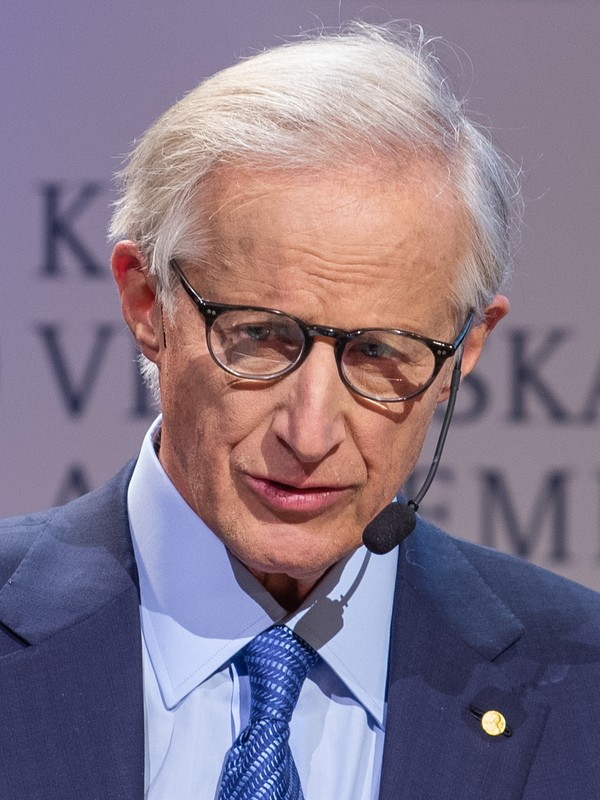
\includegraphics[width=0.48\linewidth,height=0.64\linewidth]{images/nordhaus.jpg} &
%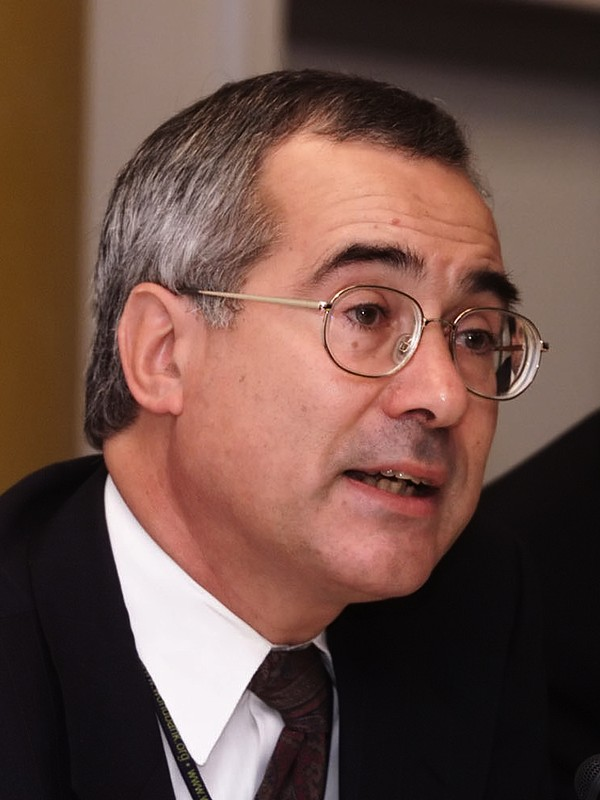
\includegraphics[width=0.48\linewidth,height=0.64\linewidth]{images/stern.jpg} \\
%{\scriptsize Nordhaus} & {\scriptsize Stern}
%\end{tabular}\\[0.5ex]
%{\fontsize{4}{5}\selectfont Photos: B. Nyman, CC BY 2.0; IMF}}}%
%BeginExpansion
\centering\setlength{\tabcolsep}{1pt}%
\begin{tabular}{cc}
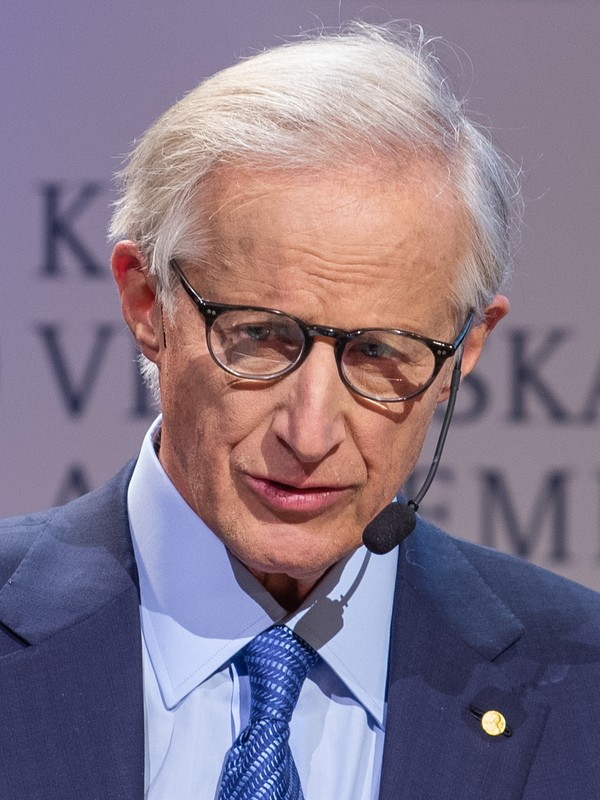
\includegraphics[width=0.48\linewidth,height=0.64\linewidth]{images/nordhaus.jpg} &
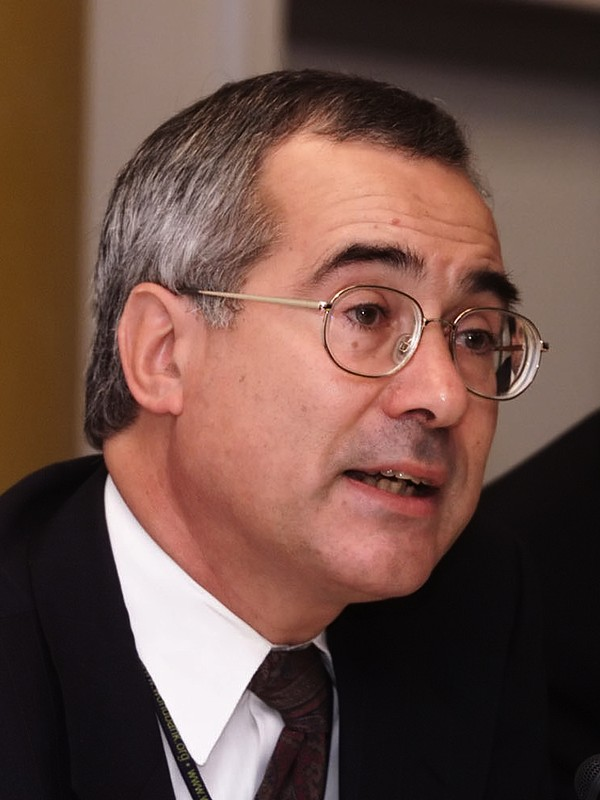
\includegraphics[width=0.48\linewidth,height=0.64\linewidth]{images/stern.jpg} \\
{\scriptsize Nordhaus} & {\scriptsize Stern}
\end{tabular}\\[0.5ex]
{\fontsize{4}{5}\selectfont Photos: B. Nyman, CC BY 2.0; IMF}%
%EndExpansion
%TCIMACRO{\TeXButton{EndColumns}{\end{columns}}}%
%BeginExpansion
\end{columns}%
%EndExpansion

%

%TCIMACRO{\TeXButton{Transition: Box Out}{\transboxout}}%
%BeginExpansion
\transboxout
%EndExpansion%
%TCIMACRO{\TeXButton{EndFrame}{\end{frame}}}%
%BeginExpansion
\end{frame}%
%EndExpansion
%

%TCIMACRO{\TeXButton{BeginFrame}{\begin{frame}}}%
%BeginExpansion
\begin{frame}%
%EndExpansion
%

%TCIMACRO{\QTR{frametitle}{The Discount Factor Controversy}}%
%BeginExpansion
\frametitle{The Discount Factor Controversy}%
%EndExpansion


\begin{stepitemizewithalert}
\item What's discount factor? Welfare function as a discounted sum of future
gains:%
\[
\mathcal{W}_{t}=L_{t}U\left(  c_{t}\right)  +\beta_{\Delta}\mathcal{W}%
_{t+\Delta}%
\]%
%TCIMACRO{\TeXButton{vspace}{\vspace{2ex}}}%
%BeginExpansion
\vspace{2ex}%
%EndExpansion


\item $\beta_{\Delta}$ is a reduced-form parameter: a single number summarizing
several distinct motives for weighting the future:%
%TCIMACRO{\TeXButton{vspace}{\vspace{2ex}}}%
%BeginExpansion
\vspace{2ex}%
%EndExpansion


\begin{stepenumeratewithalert}
\item psychological aspects (time-preference $\rightarrow\beta_{\Delta}$
low),
%TCIMACRO{\TeXButton{vspace}{\vspace{1.5ex}}}%
%BeginExpansion
\vspace{1.5ex}%
%EndExpansion


\item political aspects (how policymakers weight the future $\rightarrow
\beta_{\Delta}$ low/high),%
%TCIMACRO{\TeXButton{vspace}{\vspace{1.5ex}}}%
%BeginExpansion
\vspace{1.5ex}%
%EndExpansion


\item intergenerational aspects (how we weight future generation welfare
$\rightarrow\beta_{\Delta}$ high).
\end{stepenumeratewithalert}
\end{stepitemizewithalert}

%

%TCIMACRO{\TeXButton{Transition: Box Out}{\transboxout}}%
%BeginExpansion
\transboxout
%EndExpansion%
%TCIMACRO{\TeXButton{EndFrame}{\end{frame}}}%
%BeginExpansion
\end{frame}%
%EndExpansion
%

%TCIMACRO{\TeXButton{BeginFrame}{\begin{frame}}}%
%BeginExpansion
\begin{frame}%
%EndExpansion
%

%TCIMACRO{\QTR{frametitle}{The Discount Factor Controversy}}%
%BeginExpansion
\frametitle{The Discount Factor Controversy}%
%EndExpansion


\begin{stepitemizewithalert}
\item In practice, $\beta_{\Delta}$ not observable, but can be inferred from
financial markets.%
%TCIMACRO{\TeXButton{vspace}{\vspace{1.5ex}}}%
%BeginExpansion
\vspace{1.5ex}%
%EndExpansion


\item Introducing a one-period financial claim:%
\begin{gather*}
\max_{\{c_{t},b_{t}\}}\sum_{i=0}^{\infty}\beta_{\Delta}^{\,i}\frac{c_{t+\Delta
i}^{1-\gamma}}{1-\gamma}+\lambda_{t}\text{ }\left[  b_{t}\left(
1+r_{t-\Delta}\right)  -c_{t}-b_{t}\right]  \\
\beta\frac{c_{t+\Delta}^{-\gamma}}{c_{t}^{-\gamma}}\left(  1+r_{t}\right)
=1\rightarrow\ln\beta_{\Delta}=\gamma\ln g+\ln r
\end{gather*}


\item By observing consumption growth and real interest rate, we can pin down
$\beta_{\Delta}$;%
%TCIMACRO{\TeXButton{vspace}{\vspace{1.5ex}}}%
%BeginExpansion
\vspace{1.5ex}%
%EndExpansion


\item But definition of relevant interest rate not clear: nominal
bonds?\ corporate bonds?%
\end{stepitemizewithalert}

%

%TCIMACRO{\TeXButton{Transition: Box Out}{\transboxout}}%
%BeginExpansion
\transboxout
%EndExpansion%
%TCIMACRO{\TeXButton{EndFrame}{\end{frame}}}%
%BeginExpansion
\end{frame}%
%EndExpansion
%

%TCIMACRO{\TeXButton{BeginFrame}{\begin{frame}}}%
%BeginExpansion
\begin{frame}%
%EndExpansion
%

%TCIMACRO{\QTR{frametitle}{The Discount Factor Controversy (cont.)}}%
%BeginExpansion
\frametitle{The Discount Factor Controversy (cont.)}%
%EndExpansion


\begin{stepitemizewithalert}
\item Nordhaus picks the market return on capital (corporate rates, about
$3\%$ real) and calibrates $\rho=1.5\%$, i.e.\ $\beta_{\Delta=1}=1/1.015\simeq
0.985$;%
%TCIMACRO{\TeXButton{vspace}{\vspace{1.5ex}}}%
%BeginExpansion
\vspace{1.5ex}%
%EndExpansion


\item \cite{stern2006stern} argues that discount factor should be
\frame{$\beta_{\Delta=1}=0.999$} (versus $0.9852$ in Nordhaus).
\end{stepitemizewithalert}

\medskip
Nordhaus\'s calibration of $\rho$ across DICE vintages:

\begin{center}%
\begin{tabular}[c]{lcc}
\toprule & $\rho$ & $\beta_{\Delta=1}=1/(1+\rho)$\\
\midrule DICE-1994 & $3.0\%$ & $0.9709$\\
DICE-2007--2016 & $1.5\%$ & $0.9852$\\
DICE-2023 & $1.0\%$ & $0.9901$\\
\midrule Stern (2006), for contrast & $0.1\%$ & $0.9990$\\
\bottomrule
\end{tabular}
\end{center}

%

%TCIMACRO{\TeXButton{Transition: Box Out}{\transboxout}}%
%BeginExpansion
\transboxout
%EndExpansion%
%TCIMACRO{\TeXButton{EndFrame}{\end{frame}}}%
%BeginExpansion
\end{frame}%
%EndExpansion
%

%TCIMACRO{\TeXButton{BeginFrame}{\begin{frame}}}%
%BeginExpansion
\begin{frame}%
%EndExpansion
%

%TCIMACRO{\QTR{frametitle}{The discount factor}}%
%BeginExpansion
\frametitle{The discount factor}%
%EndExpansion


\begin{stepitemizewithalert}
\item The \cite{stern2006stern}'s report provides a scientific motivation for
the Paris-Agreement.
%TCIMACRO{\TeXButton{vspace}{\vspace{1.5ex}}}%
%BeginExpansion
\vspace{1.5ex}%
%EndExpansion


\item How? Consider FOC on\ T:%
\begin{align*}
\lambda_{4,t} &  =\beta_{\Delta}\left[  \Phi_{T}^{\top}\lambda_{4,t+\Delta
}+\lambda_{2,t+\Delta}s_{t+\Delta}Y_{t+\Delta}\left(  1-\theta_{1,t+\Delta}%
\mu_{t+\Delta}^{\theta_{2}}\right)  \nabla_{T}\Omega\left(  T_{t}\right)
\right]  \\
&  =\sum\limits_{i=1}^{\infty}\left(  \beta_{\Delta}\Phi_{T}^{\top}\right)
^{i}s_{t+\Delta i}Y_{t+\Delta i}\left(  1-\theta_{1,t+\Delta i}\mu_{t+\Delta
i}^{\theta_{2}}\right)  \nabla_{T}\Omega\left(  T_{t+\Delta\left(  i-1\right)
}\right)
\end{align*}%
%TCIMACRO{\TeXButton{vspace}{\vspace{1.5ex}}}%
%BeginExpansion
\vspace{1.5ex}%
%EndExpansion


\item Bigger $\beta$\ raises the weight $\beta_{\Delta}^{i}$ on future marginal
damages $\nabla_{T}\Omega$ in the shadow value of temperature $\lambda_{4,t}$
$\rightarrow$ larger weight for future generations, SCC $\nearrow$
\end{stepitemizewithalert}

%

%TCIMACRO{\TeXButton{Transition: Box Out}{\transboxout}}%
%BeginExpansion
\transboxout
%EndExpansion%
%TCIMACRO{\TeXButton{EndFrame}{\end{frame}}}%
%BeginExpansion
\end{frame}%
%EndExpansion


\section{The Damage Function and Tipping Points}%

%TCIMACRO{\TeXButton{BeginFrame}{\begin{frame}}}%
%BeginExpansion
\begin{frame}%
%EndExpansion
%

%TCIMACRO{\QTR{frametitle}{Damage functions: Nordhaus vs.\ Weitzman}}%
%BeginExpansion
\frametitle{Damage functions: Nordhaus vs.\ Weitzman}%
%EndExpansion


Share of output left after climate damages, $\Omega(T)$, up to $7%
%TCIMACRO{\U{b0}}%
%BeginExpansion
{{}^\circ}%
%EndExpansion
$C:%
%TCIMACRO{\TeXButton{vspace}{\vspace{1ex}}}%
%BeginExpansion
\vspace{1ex}%
%EndExpansion


%TCIMACRO{\TeXButton{Damage plot}{\begin{center}
%\begin{tikzpicture}
%\begin{axis}[width=0.78\textwidth,height=5.6cm,
%xmin=0,xmax=7,ymin=0.2,ymax=1.02,domain=0:7,samples=141,
%xlabel={Atmospheric temperature $T^{AT}$ ($^{\circ}$C above preindustrial)},
%ylabel={$\Omega(T)$},legend pos=south west,legend cell align=left,
%grid=major,grid style={gray!20},label style={font=\small},
%tick label style={font=\footnotesize},legend style={font=\footnotesize}]
%\addplot[ssp2,very thick]{1/(1+0.00236*x^2)};
%\addlegendentry{$b=0$: Nordhaus (2017)}
%\addplot[ssp5,very thick,dashed]{1/(1+0.00236*x^2+5.0703e-6*x^6.754)};
%\addlegendentry{$b>0$: Weitzman (2012)}
%\end{axis}
%\end{tikzpicture}
%\end{center}}}%
%BeginExpansion
\begin{center}
\begin{tikzpicture}
\begin{axis}[width=0.78\textwidth,height=5.6cm,
xmin=0,xmax=7,ymin=0.2,ymax=1.02,domain=0:7,samples=141,
xlabel={Atmospheric temperature $T^{AT}$ ($^{\circ}$C above preindustrial)},
ylabel={$\Omega(T)$},legend pos=south west,legend cell align=left,
grid=major,grid style={gray!20},label style={font=\small},
tick label style={font=\footnotesize},legend style={font=\footnotesize}]
\addplot[ssp2,very thick]{1/(1+0.00236*x^2)};
\addlegendentry{$b=0$: Nordhaus (2017)}
\addplot[ssp5,very thick,dashed]{1/(1+0.00236*x^2+5.0703e-6*x^6.754)};
\addlegendentry{$b>0$: Weitzman (2012)}
\end{axis}
\end{tikzpicture}
\end{center}%
%EndExpansion


%

%TCIMACRO{\TeXButton{Transition: Box Out}{\transboxout}}%
%BeginExpansion
\transboxout
%EndExpansion%
%TCIMACRO{\TeXButton{EndFrame}{\end{frame}}}%
%BeginExpansion
\end{frame}%
%EndExpansion
%

%TCIMACRO{\TeXButton{BeginFrame}{\begin{frame}}}%
%BeginExpansion
\begin{frame}%
%EndExpansion
%

%TCIMACRO{\QTR{frametitle}{Tipping points}}%
%BeginExpansion
\frametitle{Tipping points}%
%EndExpansion


\begin{stepitemizewithalert}
\item Tipping point are critical threshold beyond which a system reorganizes
abruptly \& irreversibly.%
%TCIMACRO{\TeXButton{vspace}{\vspace{1.5ex}}}%
%BeginExpansion
\vspace{1.5ex}%
%EndExpansion


\item Natural system tipping points well identified:

\begin{itemize}
\item \textsf{Antarctic \& Artic ice sheet disintegration:} complete
disintegration (at +10$%
%TCIMACRO{\U{b0}}%
%BeginExpansion
{{}^\circ}%
%EndExpansion
$C) would raise the global sea levels by 53.3 metres;

\item \textsf{Amazon Rainforest destruction: }a warming planet $\rightarrow
$rainforest may transform into a dry savanna landscape;

\item \textsf{Sibera's Permafrost thaw:} unfreezing permafrost would release
methane $\nearrow$ T$%
%TCIMACRO{\U{b0}}%
%BeginExpansion
{{}^\circ}%
%EndExpansion
C$.

\item etc.%
%TCIMACRO{\TeXButton{vspace}{\vspace{1.5ex}}}%
%BeginExpansion
\vspace{1.5ex}%
%EndExpansion

\end{itemize}

\item Tipping points are possible at today's global warming of just over 1
%TCIMACRO{\U{b0}}%
%BeginExpansion
${{}^\circ}$%
%EndExpansion
C (1.8
%TCIMACRO{\U{b0}}%
%BeginExpansion
${{}^\circ}$%
%EndExpansion
F) above preindustrial times, and highly probable above 2
%TCIMACRO{\U{b0}}%
%BeginExpansion
${{}^\circ}$%
%EndExpansion
C (3.6
%TCIMACRO{\U{b0}}%
%BeginExpansion
${{}^\circ}$%
%EndExpansion
F) of global warming.
\end{stepitemizewithalert}

%

%TCIMACRO{\TeXButton{Transition: Box Out}{\transboxout}}%
%BeginExpansion
\transboxout
%EndExpansion%
%TCIMACRO{\TeXButton{EndFrame}{\end{frame}}}%
%BeginExpansion
\end{frame}%
%EndExpansion
%

%TCIMACRO{\TeXButton{BeginFrame}{\begin{frame}}}%
%BeginExpansion
\begin{frame}%
%EndExpansion
%

%TCIMACRO{\QTR{frametitle}{Tipping points}}%
%BeginExpansion
\frametitle{Tipping points}%
%EndExpansion


\begin{stepitemizewithalert}
\item Tipping point are critical threshold beyond which a system reorganizes
abruptly \& irreversibly.%
%TCIMACRO{\TeXButton{vspace}{\vspace{1.5ex}}}%
%BeginExpansion
\vspace{1.5ex}%
%EndExpansion


\item The damage function in \cite{nordhaus2017revisiting} augmented by
\cite{weitzman2012ghg} with higher order polynomial:%
\[
\Omega\left(  T_{t}\right)  =1/(1+a_{2}\left(  T_{t}^{AT}\right)  ^{2}%
+bT_{t}^{c})
\]
where $b$ and $c$ are set to match potential losses as $T$\ grows:
$b=5.0703e-06$, $c=6.754$.%
%TCIMACRO{\TeXButton{vspace}{\vspace{1.5ex}}}%
%BeginExpansion
\vspace{1.5ex}%
%EndExpansion

\end{stepitemizewithalert}

\begin{center}%
\begin{tabular}
[c]{llll}\cline{2-4}
& $\Omega\left(  1\right)  $ & $\Omega\left(  3\right)  $ & $\Omega\left(
5\right)  $\\\hline
$b=0$ - \cite{nordhaus2017revisiting} & 0.9976 & 0.9792 & 0.9443\\
$b>0$ - \cite{weitzman2012ghg} & 0.9976 & 0.9712 & 0.7544\\\hline
\end{tabular}



\end{center}

%

%TCIMACRO{\TeXButton{Transition: Box Out}{\transboxout}}%
%BeginExpansion
\transboxout
%EndExpansion%
%TCIMACRO{\TeXButton{EndFrame}{\end{frame}}}%
%BeginExpansion
\end{frame}%
%EndExpansion
%

%TCIMACRO{\TeXButton{BeginFrame}{\begin{frame}}}%
%BeginExpansion
\begin{frame}%
%EndExpansion
%

%TCIMACRO{\QTR{frametitle}{Tipping points}}%
%BeginExpansion
\frametitle{Tipping points}%
%EndExpansion


\begin{stepitemizewithalert}
\item Why tipping points call for stronger actions?%
%TCIMACRO{\TeXButton{vspace}{\vspace{1.5ex}}}%
%BeginExpansion
\vspace{1.5ex}%
%EndExpansion


\item Get back to FOC:%
\[
\lambda_{4,t}^{AT}=\sum\limits_{i=1}^{\infty}\left(  \beta_{\Delta}\Phi
_{T}^{\top}\right)  ^{i}s_{t+\Delta i}Y_{t+\Delta i}\left(  1-\theta
_{1,t+\Delta i}\mu_{t+\Delta i}^{\theta_{2}}\right)  \nabla_{T}\Omega\left(
T_{t+\Delta\left(  i-1\right)  }\right)
\]%
%TCIMACRO{\TeXButton{vspace}{\vspace{0.5ex}}}%
%BeginExpansion
\vspace{0.5ex}%
%EndExpansion


\item $\nabla_{T}\Omega\left(  T_{t+\Delta\left(  i-1\right)  }\right)  $ much
larger under tipping climate, thus rising the Social Cost of Carbon and in
turn the carbon tax.
\end{stepitemizewithalert}

%

%TCIMACRO{\TeXButton{Transition: Box Out}{\transboxout}}%
%BeginExpansion
\transboxout
%EndExpansion%
%TCIMACRO{\TeXButton{EndFrame}{\end{frame}}}%
%BeginExpansion
\end{frame}%
%EndExpansion


\section{Estimating damages: global vs.\ local temperature}%

%TCIMACRO{\TeXButton{BeginFrame}{\begin{frame}}}%
%BeginExpansion
\begin{frame}%
%EndExpansion
%

%TCIMACRO{\QTR{frametitle}{Empirical damages: global vs.\ local temperature}}%
%BeginExpansion
\frametitle{Empirical damages: global vs.\ local temperature}%
%EndExpansion


\begin{stepitemizewithalert}
\item The damage function is the weakest link of IAMs: $a_{2}$ is calibrated, not
estimated $\rightarrow$ can we \textbf{estimate} it from macro data?%
%TCIMACRO{\TeXButton{vspace}{\vspace{1.5ex}}}%
%BeginExpansion
\vspace{1.5ex}%
%EndExpansion


\item \cite{bilal2026macroeconomic}: shift the focus from \textbf{local} to
\textbf{global} temperature:
\begin{stepenumeratewithalert}
\item a $1%
%TCIMACRO{\U{b0}}%
%BeginExpansion
{{}^\circ}%
%EndExpansion
$C global warming lowers world GDP by \textbf{over 20\%} in the long run,
an order of magnitude more than with country-level temperature;%
%TCIMACRO{\TeXButton{vspace}{\vspace{1ex}}}%
%BeginExpansion
\vspace{1ex}%
%EndExpansion


\item global temperature correlates strongly with \textbf{extreme events},
country-level temperature does not.
\end{stepenumeratewithalert}%
%TCIMACRO{\TeXButton{vspace}{\vspace{1.5ex}}}%
%BeginExpansion
\vspace{1.5ex}%
%EndExpansion


\item Feeding the estimated damage function into a neoclassical growth model:
business-as-usual welfare loss \textbf{above 30\%}, SCC \textbf{above
\$1\,200/tCO$_{2}$}.
\end{stepitemizewithalert}

%

%TCIMACRO{\TeXButton{Transition: Box Out}{\transboxout}}%
%BeginExpansion
\transboxout
%EndExpansion%
%TCIMACRO{\TeXButton{EndFrame}{\end{frame}}}%
%BeginExpansion
\end{frame}%
%EndExpansion
%

%TCIMACRO{\TeXButton{BeginFrame}{\begin{frame}}}%
%BeginExpansion
\begin{frame}%
%EndExpansion
%

%TCIMACRO{\QTR{frametitle}{Global temperature and world GDP: two trending series}}%
%BeginExpansion
\frametitle{Global temperature and world GDP: two trending series}%
%EndExpansion


%TCIMACRO{\TeXButton{Figure}{\centering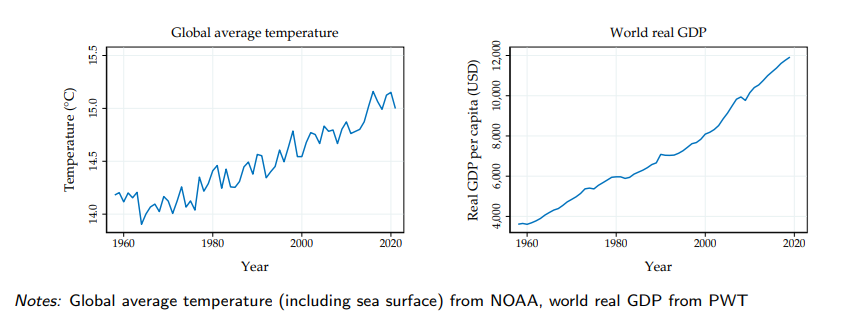
\includegraphics[width=0.8\linewidth]{images/kanzig1.png}}}%
%BeginExpansion
\centering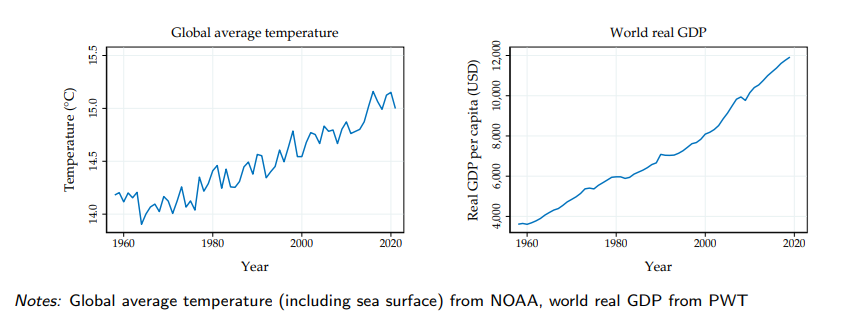
\includegraphics[width=0.8\linewidth]{images/kanzig1.png}%
%EndExpansion

\begin{stepitemizewithalert}
\item Both global temperature and world GDP \textbf{trend upward}.%
%TCIMACRO{\TeXButton{vspace}{\vspace{1ex}}}%
%BeginExpansion
\vspace{1ex}%
%EndExpansion


\item Regressing one on the other $\rightarrow$ risk of \textbf{spurious
correlation}.%
%TCIMACRO{\TeXButton{vspace}{\vspace{1ex}}}%
%BeginExpansion
\vspace{1ex}%
%EndExpansion


\item Solution: focus on \textbf{temperature shocks}, i.e.\ transitory deviations
around the trend.
\end{stepitemizewithalert}

%

%TCIMACRO{\TeXButton{Transition: Box Out}{\transboxout}}%
%BeginExpansion
\transboxout
%EndExpansion%
%TCIMACRO{\TeXButton{EndFrame}{\end{frame}}}%
%BeginExpansion
\end{frame}%
%EndExpansion
%

%TCIMACRO{\TeXButton{BeginFrame}{\begin{frame}}}%
%BeginExpansion
\begin{frame}%
%EndExpansion
%

%TCIMACRO{\QTR{frametitle}{Measuring temperature shocks}}%
%BeginExpansion
\frametitle{Measuring temperature shocks}%
%EndExpansion


\begin{stepitemizewithalert}
\item Following \textbf{Hamilton (2018)}: the shock is the \textbf{forecast error}
of temperature:%
\[
\widehat{T}_{t+h}^{\text{shock}}=T_{t+h}-\left(  \hat{\beta}_{0}+\hat{\beta}_{1}T_{t}+\cdots+\hat{\beta}_{p}T_{t-p+1}\right)
\]%
%TCIMACRO{\TeXButton{vspace}{\vspace{1.5ex}}}%
%BeginExpansion
\vspace{1.5ex}%
%EndExpansion


\item Sources of variation around the trend:
\begin{stepenumeratewithalert}
\item exogenous drivers: solar cycles, volcanic eruptions;%
%TCIMACRO{\TeXButton{vspace}{\vspace{1ex}}}%
%BeginExpansion
\vspace{1ex}%
%EndExpansion


\item internal climate variability: ocean circulation, El Ni\~{n}o.
\end{stepenumeratewithalert}%
%TCIMACRO{\TeXButton{vspace}{\vspace{1.5ex}}}%
%BeginExpansion
\vspace{1.5ex}%
%EndExpansion


\item $h=2$, $p=2$ to capture \textbf{persistent} climate phenomena (e.g.\ El
Ni\~{n}o); results robust to other specifications.
\end{stepitemizewithalert}

%

%TCIMACRO{\TeXButton{Transition: Box Out}{\transboxout}}%
%BeginExpansion
\transboxout
%EndExpansion%
%TCIMACRO{\TeXButton{EndFrame}{\end{frame}}}%
%BeginExpansion
\end{frame}%
%EndExpansion
%

%TCIMACRO{\TeXButton{BeginFrame}{\begin{frame}}}%
%BeginExpansion
\begin{frame}%
%EndExpansion
%

%TCIMACRO{\QTR{frametitle}{Exogenous temperature shocks}}%
%BeginExpansion
\frametitle{Exogenous temperature shocks}%
%EndExpansion


%TCIMACRO{\TeXButton{Figure}{\centering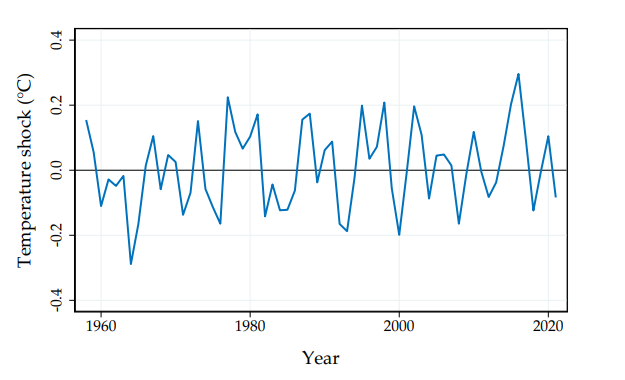
\includegraphics[width=0.62\linewidth]{images/kanzig2.png}}}%
%BeginExpansion
\centering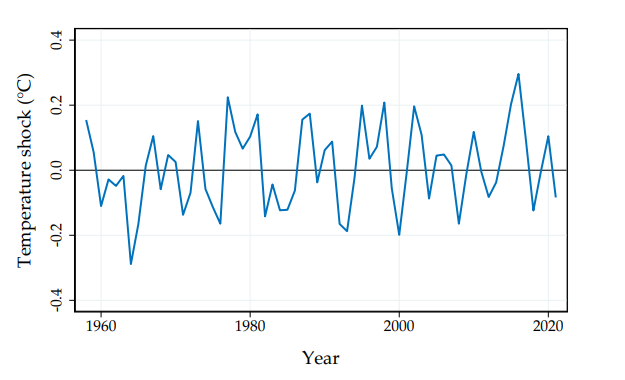
\includegraphics[width=0.62\linewidth]{images/kanzig2.png}%
%EndExpansion

%

%TCIMACRO{\TeXButton{Transition: Box Out}{\transboxout}}%
%BeginExpansion
\transboxout
%EndExpansion%
%TCIMACRO{\TeXButton{EndFrame}{\end{frame}}}%
%BeginExpansion
\end{frame}%
%EndExpansion
%

%TCIMACRO{\TeXButton{BeginFrame}{\begin{frame}}}%
%BeginExpansion
\begin{frame}%
%EndExpansion
%

%TCIMACRO{\QTR{frametitle}{Estimating the effects of global temperature shocks}}%
%BeginExpansion
\frametitle{Estimating the effects of global temperature shocks}%
%EndExpansion


\begin{stepitemizewithalert}
\item Dynamic causal effects estimated by \textbf{local projections}
(Jord\`{a}, 2005):%
\[
y_{t+h}-y_{t-1}=\alpha_{h}+\theta_{h}T_{t}^{\text{shock}}+\mathbf{x}_{t}^{\prime}\boldsymbol{\beta}_{h}+\varepsilon_{t+h}
\]%
%TCIMACRO{\TeXButton{vspace}{\vspace{1.5ex}}}%
%BeginExpansion
\vspace{1.5ex}%
%EndExpansion


\item $y_{t}$: log real world GDP per capita; $T_{t}^{\text{shock}}$: global
temperature shock; $\mathbf{x}_{t}$: controls.%
%TCIMACRO{\TeXButton{vspace}{\vspace{1.5ex}}}%
%BeginExpansion
\vspace{1.5ex}%
%EndExpansion


\item $\theta_{h}$: \textbf{causal effect at horizon} $h$ $\rightarrow$ the
sequence $\{\theta_{h}\}$ traces the impulse response of GDP.
\end{stepitemizewithalert}

%

%TCIMACRO{\TeXButton{Transition: Box Out}{\transboxout}}%
%BeginExpansion
\transboxout
%EndExpansion%
%TCIMACRO{\TeXButton{EndFrame}{\end{frame}}}%
%BeginExpansion
\end{frame}%
%EndExpansion
%

%TCIMACRO{\TeXButton{BeginFrame}{\begin{frame}}}%
%BeginExpansion
\begin{frame}%
%EndExpansion
%

%TCIMACRO{\QTR{frametitle}{Effects of global temperature shocks}}%
%BeginExpansion
\frametitle{Effects of global temperature shocks}%
%EndExpansion


%TCIMACRO{\TeXButton{BeginColumns}{\begin{columns}}}%
%BeginExpansion
\begin{columns}%
%EndExpansion
%TCIMACRO{\TeXButton{Column}{\column{0.52\textwidth}}}%
%BeginExpansion
\column{0.52\textwidth}%
%EndExpansion
%TCIMACRO{\TeXButton{Figure}{\centering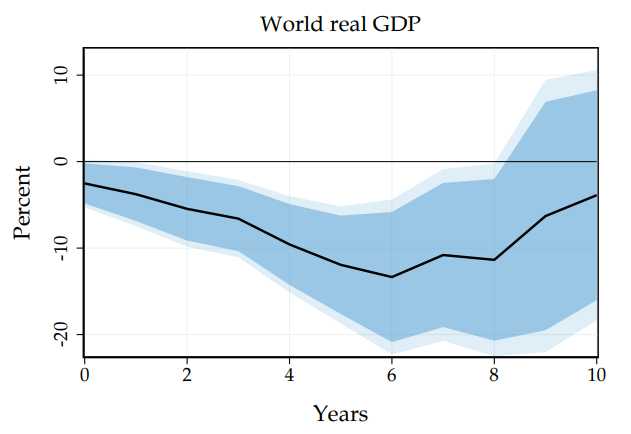
\includegraphics[width=1\linewidth]{images/kanzig3.png}}}%
%BeginExpansion
\centering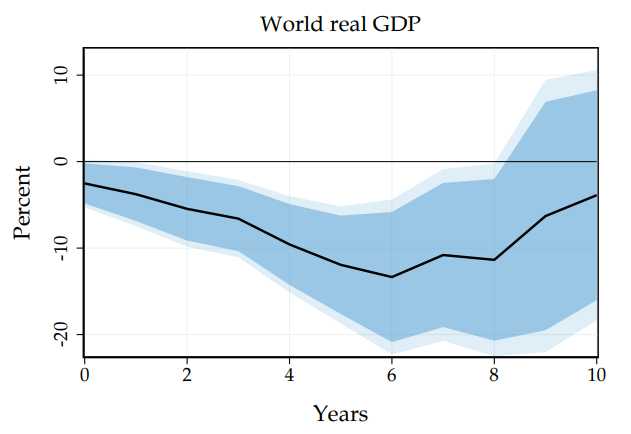
\includegraphics[width=1\linewidth]{images/kanzig3.png}%
%EndExpansion
%TCIMACRO{\TeXButton{Notes}{\par{\footnotesize\raggedright\textit{Notes}: 90\% and 95\% confidence bands, robust standard errors.\par}}}%
%BeginExpansion
\par{\footnotesize\raggedright\textit{Notes}: 90\% and 95\% confidence bands, robust standard errors.\par}%
%EndExpansion

%TCIMACRO{\TeXButton{Column}{\column{0.46\textwidth}}}%
%BeginExpansion
\column{0.46\textwidth}%
%EndExpansion

\begin{stepitemizewithalert}
\item Significant and \textbf{persistent} effect.%
%TCIMACRO{\TeXButton{vspace}{\vspace{1ex}}}%
%BeginExpansion
\vspace{1ex}%
%EndExpansion


\item After a $1%
%TCIMACRO{\U{b0}}%
%BeginExpansion
{{}^\circ}%
%EndExpansion
$C shock:
\begin{stepenumeratewithalert}
\item GDP per capita falls by \textbf{2\%} on impact;%
%TCIMACRO{\TeXButton{vspace}{\vspace{0.5ex}}}%
%BeginExpansion
\vspace{0.5ex}%
%EndExpansion


\item the effect exceeds \textbf{10\%} after 6 years;%
%TCIMACRO{\TeXButton{vspace}{\vspace{0.5ex}}}%
%BeginExpansion
\vspace{0.5ex}%
%EndExpansion


\item still there 10 years later, driven by the \textbf{persistence of
temperature} itself.
\end{stepenumeratewithalert}
\end{stepitemizewithalert}
%TCIMACRO{\TeXButton{EndColumns}{\end{columns}}}%
%BeginExpansion
\end{columns}%
%EndExpansion

%

%TCIMACRO{\TeXButton{Transition: Box Out}{\transboxout}}%
%BeginExpansion
\transboxout
%EndExpansion%
%TCIMACRO{\TeXButton{EndFrame}{\end{frame}}}%
%BeginExpansion
\end{frame}%
%EndExpansion
%

%TCIMACRO{\TeXButton{BeginFrame}{\begin{frame}}}%
%BeginExpansion
\begin{frame}%
%EndExpansion
%

%TCIMACRO{\QTR{frametitle}{A climate--economy panel}}%
%BeginExpansion
\frametitle{A climate--economy panel}%
%EndExpansion


\begin{stepitemizewithalert}
\item \textbf{173 countries}, from 1960 (back to 1900 for some).%
%TCIMACRO{\TeXButton{vspace}{\vspace{1ex}}}%
%BeginExpansion
\vspace{1ex}%
%EndExpansion


\item Economic data: PWT and JST Macrohistory (GDP, population, capital,
investment, productivity); temperature: Berkeley Earth; extreme events:
ISIMIP gridded data.%
%TCIMACRO{\TeXButton{vspace}{\vspace{1ex}}}%
%BeginExpansion
\vspace{1ex}%
%EndExpansion


\item \textbf{Panel local projections} (Jord\`{a} et al., 2020):%
\[
y_{i,t+h}-y_{i,t-1}=\alpha_{i,h}+\theta_{h}T_{t}^{\text{shock}}+\mathbf{x}_{t}^{\prime}\boldsymbol{\beta}_{h}+\mathbf{x}_{i,t}^{\prime}\boldsymbol{\gamma}_{h}+\varepsilon_{i,t+h}
\]%
%TCIMACRO{\TeXButton{vspace}{\vspace{1ex}}}%
%BeginExpansion
\vspace{1ex}%
%EndExpansion


\item Allows comparing responses to \textbf{global} and \textbf{local}
temperature shocks.
\end{stepitemizewithalert}

%

%TCIMACRO{\TeXButton{Transition: Box Out}{\transboxout}}%
%BeginExpansion
\transboxout
%EndExpansion%
%TCIMACRO{\TeXButton{EndFrame}{\end{frame}}}%
%BeginExpansion
\end{frame}%
%EndExpansion
%

%TCIMACRO{\TeXButton{BeginFrame}{\begin{frame}}}%
%BeginExpansion
\begin{frame}%
%EndExpansion
%

%TCIMACRO{\QTR{frametitle}{Global temperature shocks in the panel}}%
%BeginExpansion
\frametitle{Global temperature shocks in the panel}%
%EndExpansion


%TCIMACRO{\TeXButton{BeginColumns}{\begin{columns}}}%
%BeginExpansion
\begin{columns}%
%EndExpansion
%TCIMACRO{\TeXButton{Column}{\column{0.52\textwidth}}}%
%BeginExpansion
\column{0.52\textwidth}%
%EndExpansion
%TCIMACRO{\TeXButton{Figure}{\centering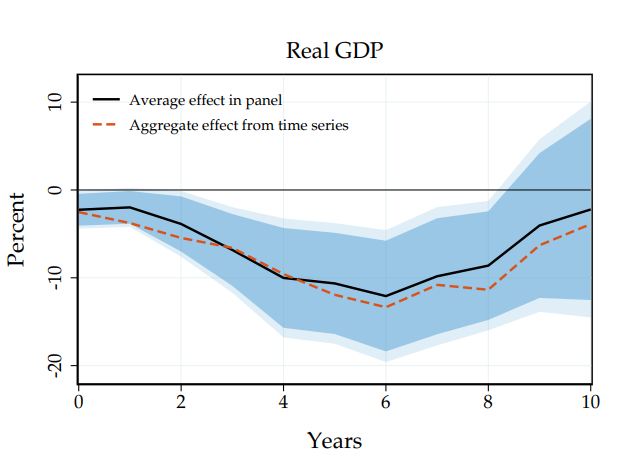
\includegraphics[width=1\linewidth]{images/kanzig4.png}}}%
%BeginExpansion
\centering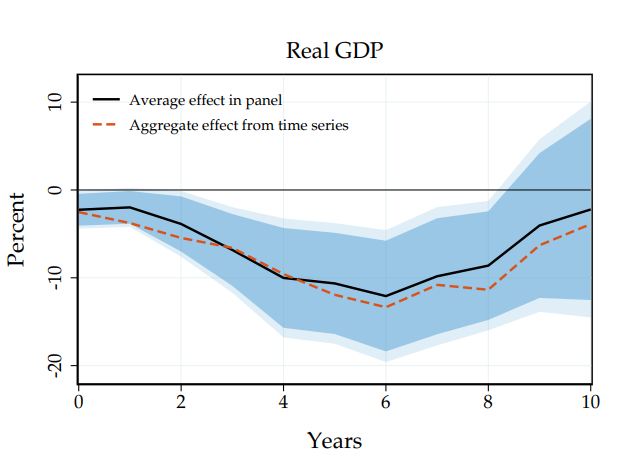
\includegraphics[width=1\linewidth]{images/kanzig4.png}%
%EndExpansion
%TCIMACRO{\TeXButton{Notes}{\par{\footnotesize\raggedright\textit{Notes}: 90\% and 95\% bands, Driscoll--Kraay standard errors.\par}}}%
%BeginExpansion
\par{\footnotesize\raggedright\textit{Notes}: 90\% and 95\% bands, Driscoll--Kraay standard errors.\par}%
%EndExpansion

%TCIMACRO{\TeXButton{Column}{\column{0.46\textwidth}}}%
%BeginExpansion
\column{0.46\textwidth}%
%EndExpansion

\begin{stepitemizewithalert}
\item \textbf{Substantial} impact: GDP per capita falls by more than
\textbf{10\%}.%
%TCIMACRO{\TeXButton{vspace}{\vspace{1.5ex}}}%
%BeginExpansion
\vspace{1.5ex}%
%EndExpansion


\item Panel effect $\approx$ time-series effect.%
%TCIMACRO{\TeXButton{vspace}{\vspace{1.5ex}}}%
%BeginExpansion
\vspace{1.5ex}%
%EndExpansion


\item Local temperature shocks: much smaller effect, in line with the earlier
literature.
\end{stepitemizewithalert}
%TCIMACRO{\TeXButton{EndColumns}{\end{columns}}}%
%BeginExpansion
\end{columns}%
%EndExpansion

%

%TCIMACRO{\TeXButton{Transition: Box Out}{\transboxout}}%
%BeginExpansion
\transboxout
%EndExpansion%
%TCIMACRO{\TeXButton{EndFrame}{\end{frame}}}%
%BeginExpansion
\end{frame}%
%EndExpansion
%

%TCIMACRO{\TeXButton{BeginFrame}{\begin{frame}}}%
%BeginExpansion
\begin{frame}%
%EndExpansion
%

%TCIMACRO{\QTR{frametitle}{Implications for IAMs}}%
%BeginExpansion
\frametitle{Implications for IAMs}%
%EndExpansion


%TCIMACRO{\TeXButton{BeginColumns}{\begin{columns}}}%
%BeginExpansion
\begin{columns}%
%EndExpansion
%TCIMACRO{\TeXButton{Column}{\column{0.56\textwidth}}}%
%BeginExpansion
\column{0.56\textwidth}%
%EndExpansion
%TCIMACRO{\TeXButton{Figure}{\centering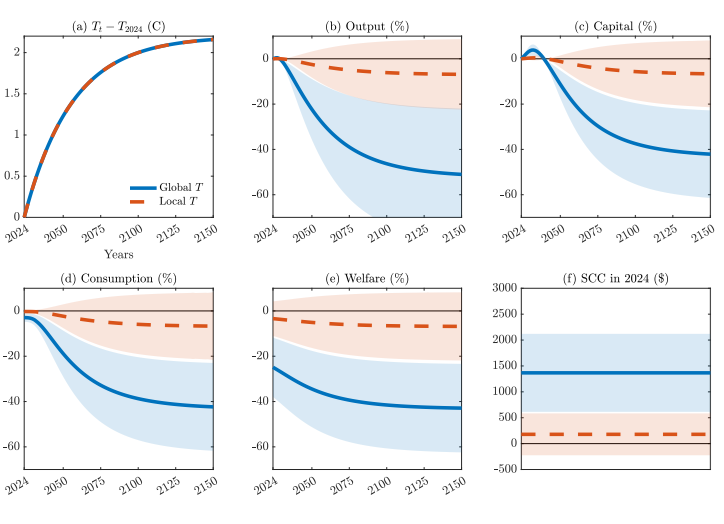
\includegraphics[width=1\linewidth]{images/kanzig5.png}}}%
%BeginExpansion
\centering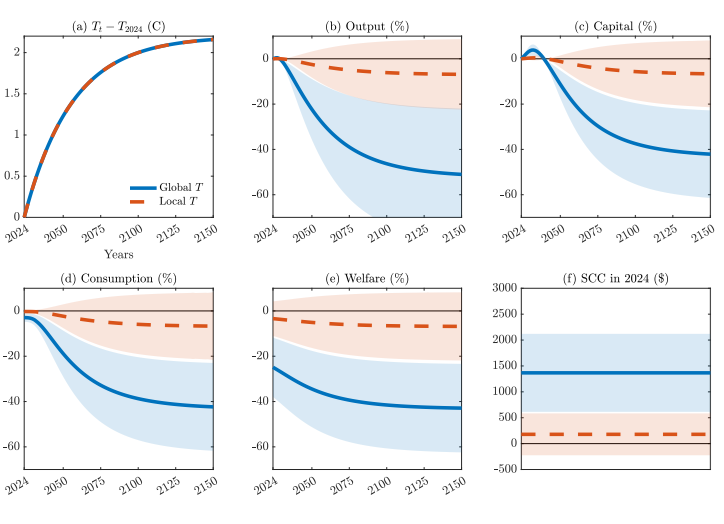
\includegraphics[width=1\linewidth]{images/kanzig5.png}%
%EndExpansion
%TCIMACRO{\TeXButton{Notes}{\par{\footnotesize\raggedright\textit{Notes}: simulated impact of global vs.\ local temperature damages, model calibrated in 2024.\par}}}%
%BeginExpansion
\par{\footnotesize\raggedright\textit{Notes}: simulated impact of global vs.\ local temperature damages, model calibrated in 2024.\par}%
%EndExpansion

%TCIMACRO{\TeXButton{Column}{\column{0.42\textwidth}}}%
%BeginExpansion
\column{0.42\textwidth}%
%EndExpansion

\begin{stepitemizewithalert}
\item \textbf{Global} damages: in 2100, $C$ and $Y$ $-40\%$; welfare loss
$25\%$; SCC $=\$1\,367$/tCO$_{2}$.%
%TCIMACRO{\TeXButton{vspace}{\vspace{1ex}}}%
%BeginExpansion
\vspace{1ex}%
%EndExpansion


\item \textbf{Local} damages: $C$ and $Y$ $-6\%$; welfare loss $3\%$; SCC
$=\$178$/tCO$_{2}$, close to standard IAMs.%
%TCIMACRO{\TeXButton{vspace}{\vspace{1ex}}}%
%BeginExpansion
\vspace{1ex}%
%EndExpansion


\item Same model, different \textbf{damage evidence} $\rightarrow$ SCC $\times7$:
aggressive decarbonization becomes optimal.
\end{stepitemizewithalert}
%TCIMACRO{\TeXButton{EndColumns}{\end{columns}}}%
%BeginExpansion
\end{columns}%
%EndExpansion

%

%TCIMACRO{\TeXButton{Transition: Box Out}{\transboxout}}%
%BeginExpansion
\transboxout
%EndExpansion%
%TCIMACRO{\TeXButton{EndFrame}{\end{frame}}}%
%BeginExpansion
\end{frame}%
%EndExpansion
%

\section{Recap}%

%TCIMACRO{\TeXButton{BeginFrame}{\begin{frame}}}%
%BeginExpansion
\begin{frame}%
%EndExpansion
%

%TCIMACRO{\QTR{frametitle}{Exam Guidelines}}%
%BeginExpansion
\frametitle{Exam Guidelines}%
%EndExpansion


\begin{stepitemizewithalert}
\item \textbf{Equations:} You don't need to memorize every equation by heart.
But you should be able to recognize them if you see them, and explain their meaning.

\item \textbf{Simulations:} You don't need to know the code. What matters is
that you understand the outputs (graphs, tables, numbers) and can interpret
them correctly.

\item \textbf{MCQs:} Expect multiple-choice questions with text, equations,
and figures. The goal is to test whether you can read, interpret, and choose
the correct answer.
\end{stepitemizewithalert}

In short: focus on understanding, not rote learning.

%

%TCIMACRO{\TeXButton{Transition: Box Out}{\transboxout}}%
%BeginExpansion
\transboxout
%EndExpansion%
%TCIMACRO{\TeXButton{EndFrame}{\end{frame}}}%
%BeginExpansion
\end{frame}%
%EndExpansion
%

%TCIMACRO{\TeXButton{BeginFrame}{\begin{frame}}}%
%BeginExpansion
\begin{frame}%
%EndExpansion


\begin{center}
Thank you!

\vspace{5ex}

$\mathtt{gauthier@vermandel.fr}$
\end{center}

%

%TCIMACRO{\TeXButton{Transition: Box Out}{\transboxout}}%
%BeginExpansion
\transboxout
%EndExpansion%
%TCIMACRO{\TeXButton{EndFrame}{\end{frame}}}%
%BeginExpansion
\end{frame}%
%EndExpansion
%

%TCIMACRO{\TeXButton{FRAME}{\bibliographystyle{apalike}
%\bibliography{lucas_romie}}}%
%BeginExpansion
\bibliographystyle{apalike}
\bibliography{lucas_romie}%
%EndExpansion

\end{document}
